\documentclass[a4paper,12pt]{article}
%\documentclass[fleqn]{article}

% ---パッケージ---
\usepackage{amsmath,amssymb}    %数式用
\usepackage{tcolorbox}   %囲み枠用(tcolorboxに変更)
\usepackage{geometry}   %余白調節
\usepackage{tikz}  % ← 図を描くためのTikZパッケージ
\geometry{margin=25mm}  %余白を少し狭く
\usetikzlibrary{decorations.pathmorphing,patterns,positioning,arrows.meta} % バネ・壁の模様
\tikzset{
  block/.style = {draw, rectangle, minimum height=2em, minimum width=3em},
  sum/.style = {draw, circle, inner sep=0pt, minimum size=5mm},
  input/.style = {coordinate},
  output/.style = {coordinate}
}
\usetikzlibrary{calc}
\usepackage{pgfplots}  % ← 追加(グラフ用)
\pgfplotsset{compat=newest} % ← 推奨設定

% --- 日本語用パッケージ ---
\usepackage{luatexja}         % 日本語表示に必要
\usepackage{luatexja-fontspec} % フォント指定用

% --- フォント指定(Overleaf標準フォント)---
\setmainjfont{IPAexMincho}  % 明朝体
%\setmainjfont{IPAexGothic}  % ゴシック体にしたい場合

% --- tcolorbox の設定 ---
\tcbset{
    colframe=black,
    colback=white,         % 本文の背景(白)
    boxrule=0.8pt,
    arc=3pt,
    outer arc=3pt,
    boxsep=4pt,
    coltitle=black,
    colbacktitle=gray!20,  % タイトルの背景(グレー)
    fonttitle=\normalsize
}

\begin{document}

\noindent
\text{制御工学Ⅰ 演習① 解答}\\
\text{2025/05/21}\\
\text{Yudai}\\


% ---------------[1]--------------- 済
\noindent
1. 次の伝達関数で表されるシステムのラプラス逆変換を行え。
\vspace{-4mm}
\[
\renewcommand{\arraystretch}{3.0} % ← 行の高さ倍率を変更(1.0が標準)
\begin{tabular}{@{}rl@{\quad\quad}rl@{}}
(1) & $G_1(s) = \dfrac{1}{s^2+2s+2}$                 & (2) & $G_2(s) = \dfrac{6}{s^3+6s^2+11s+6}$ \\
\end{tabular}
\]

% ---------------[2]---------------
\noindent
2. 以下の問に答えよ。なお、システムの入力を外力\(f(t)\)、出力を変位\(x(t)\)とし、
初期状態において系は静止しているとする。

\begin{center}
  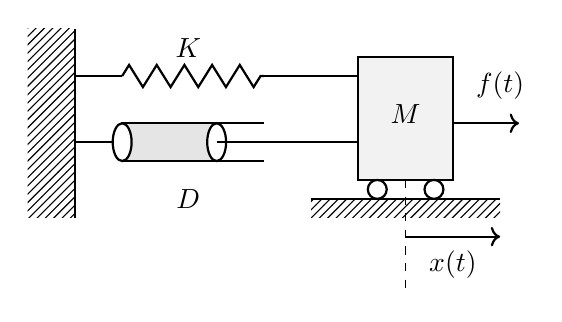
\begin{tikzpicture}[scale=1.2]
    % 固定壁
    \fill[pattern=north east lines] (-0.5,0) rectangle (0,2);
    \draw[thick] (0,0) -- (0,2);
  
    % バネ
    \draw[thick] (0,1.5) -- (0.5,1.5);
    \draw[thick, decorate, decoration={zigzag, segment length=10, amplitude=4}] (0.5,1.5) -- (2,1.5);
    \draw[thick] (2,1.5) -- (3.5,1.5);
    \node at (1.2,1.8) {$K$};
  
    % ダンパー(シリンダー形式)
    \draw[thick] (0,0.8) -- (0.5,0.8); % 棒
    \draw[thick, fill=gray!20] (0.5,0.6) rectangle (1.5,1.0); % 筒の側面
    \draw[thick] (1.5,1.0) -- (2,1.0); % 筒の上
    \draw[thick] (1.5,0.6) -- (2,0.6); % 筒の下
    \draw[thick, fill=white] (0.5,0.8) ellipse (0.1 and 0.2); % 左端面
    \draw[thick, fill=white] (1.5,0.8) ellipse (0.1 and 0.2); % 右端面
    \draw[thick] (1.5,0.8) -- (3,0.8); % ピストン棒
    \node at (1.2,0.2) {$D$};
  
    % 質量M
    \draw[thick, fill=gray!10] (3,0.4) rectangle (4,1.7);
    \node at (3.5,1.1) {$M$};
    % ローラー追加
      \draw[thick] (3.2,0.3) circle (0.1);
      \draw[thick] (3.8,0.3) circle (0.1);

  
    % 床
    \draw[thick] (2.5,0.2) -- (4.5,0.2);
    \fill[pattern=north east lines] (2.5,0) rectangle (4.5,0.2);
  
    % 座標
    \draw[->, thick] (3.5,-0.2) -- (4.5,-0.2);
    \node at (4,-0.5) {$x(t)$};
    \draw[dashed] (3.5,0.4) -- (3.5,-0.8);
  
    % 外力
    \draw[->, thick] (4,1) -- (4.7,1);
    \node at (4.5,1.4) {$f(t)$};
  \end{tikzpicture}
\end{center}

\indent
(1)上図によって示されるシステムの運動方程式ならびに伝達関数を求めよ。\\

\indent
(2)各パラメータを\(M=1,D=5,K=6\)として、インパルス応答を求めよ。\\

\indent
(3)問(2)のパラメータを用いて、単位ステップ応答\(x(t)\)を求めよ。\\

\indent
(4)単位ステップ応答の概形を描け。
なおグラフの横軸を時間\(t\),縦軸を変位\(x(t)\)とする。\\

\indent
(5)\(M=1,D=0,K=0,\)入力を\(f(t)=\sin \omega t\)として、応答\(x(t)\)を求めよ。\\

\indent
(6)\(M=1,D=0,K=2\)として、ステップ入力を与えたときの応答\(x(t)\)を求めよ。\\

\indent
(7)\(M=1,D=2,K=1,\)入力を\(f(t)=\sin \omega t\)として、応答\(x(t)\)を求めよ。\\

\indent
(8)\(M=1,D=4,K=5\)として、ステップ入力を与えたときの応答\(x(t)\)を求めよ。\\


% ---------------[3]--------------- 
\noindent
3.次の微分方程式について、初期値をすべて0として、\(x(t)\)を求めよ。\\

(1)\quad \( \ddot{x}(t)+ 2\dot{x}+ 2x(t)= \sin 2t \)\\

(2)\quad \( \dot{x}(t)+ x(t)= 1(t)- 1(t-2) \)\\



% ---------------[4]---------------
\noindent
4.下図の物理モデルにおいて、\(f(t)\)に単位ステップ入力を印加するとき、
    \(x(t)\)を求めよ。なお、\(m=9,k=1\)とし、初期値をすべて\(0\)とする。
    \begin{center}
        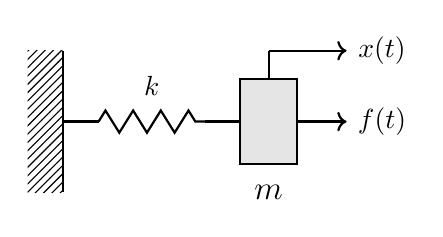
\begin{tikzpicture}[scale=0.9]
            % 固定壁
            \fill[pattern=north east lines] (-0.5,0) rectangle (0,2);
            \draw[thick] (0,0) -- (0,2);
    
            % バネ
            \draw[thick] (0,1) -- (0.5,1);
            \draw[thick, decorate, decoration={zigzag, segment length=10, amplitude=4}] (0.5,1) -- (2,1);
            \node at (1.25,1.5) {$k$};
    
            % --- 物体 ---
            \draw[thick] (2,1) -- (2.5,1); % 棒(変更なし)
            \draw[thick, fill=gray!20] (2.5,0.4) rectangle (3.3,1.6); % 筒の側面
            \node at (2.9,0) {\large $m$};
    
    
            % 入力矢印
            \draw[->, thick] (3.3,1.0) -- (4.0,1.0);
            \node at (4.5,1.0) {$f(t)$};
    
            % 出力矢印
            \draw[thick] (2.9,1.6) -- (2.9,2.0);
            \draw[->, thick] (2.9,2.0) -- (4.0,2.0);
            \node at (4.5,2.0) {$x(t)$};
    
    
        \end{tikzpicture}
    \end{center}


% ---------------[5]---------------
\noindent
5.下図に示すシステムについて、入力を変位\(x_i(t),\)出力を変位\(x_o(t)\)としたとき、
次の問に答えよ。なお、\(m\)は質量[kg]、\(d\)は粘性係数[Ns/m]、kはバネ定数[N/m]とし、
初期状態において系は静止しているとする。
  \begin{center}
    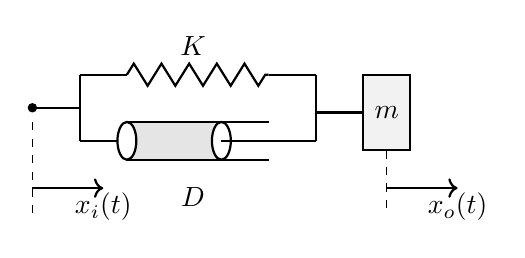
\begin{tikzpicture}[scale=1.2]
      % バネ
      \draw[thick] (0,1.5) -- (0.5,1.5);
      \draw[thick, decorate, decoration={zigzag, segment length=10, amplitude=4}] (0.5,1.5) -- (2,1.5);
      \draw[thick] (2,1.5) -- (2.5,1.5);
      \node at (1.2,1.8) {$K$};
    
      % ダンパー(シリンダー形式)
      \draw[thick] (0,0.8) -- (0.5,0.8); % 棒
      \draw[thick, fill=gray!20] (0.5,0.6) rectangle (1.5,1.0); % 筒の側面
      \draw[thick] (1.5,1.0) -- (2,1.0); % 筒の上
      \draw[thick] (1.5,0.6) -- (2,0.6); % 筒の下
      \draw[thick, fill=white] (0.5,0.8) ellipse (0.1 and 0.2); % 左端面
      \draw[thick, fill=white] (1.5,0.8) ellipse (0.1 and 0.2); % 右端面
      \draw[thick] (1.5,0.8) -- (2.5,0.8); % ピストン棒
      \node at (1.2,0.2) {$D$};

      %接続部分
      \draw[thick] (2.5,1.5) -- (2.5,0.8);
      \draw[thick] (2.5,1.1) -- (3.0,1.1);

      % 質量m
      \draw[thick, fill=gray!10] (3,0.7) rectangle (3.5,1.5);
      \node at (3.25,1.1) {$m$};

      % 座標
      \draw[->, thick] (3.25,0.3) -- (4,0.3);
      \node at (4,0.1) {$x_o(t)$};
      \draw[dashed] (3.25,0.7) -- (3.25,0);

      \draw[->, thick] (-0.5,0.3) -- (0.25,0.3);
      \node at (0.25,0.1) {$x_i(t)$};
      \draw[dashed] (-0.5,1) -- (-0.5,0);

      \draw[thick] (0,0.8) -- (0,1.5);
      \draw[thick] (0,1.15) -- (-0.5,1.15);

      \fill (-0.5,1.15) circle (0.05);
    \end{tikzpicture}
  \end{center}

\indent
(1)システムの運動方程式を求めよ。\\

\indent
(2)システムの伝達関数を求めよ。\\

\indent
(3)インパルス入力を印加した際の定常値を求めよ。\\

\indent
(4)ステップ入力を印加した際の定常値を求めよ。\\

\indent
(5)\quad \( m=1,d=3,k=2\)とし、インパルス応答、ステップ応答をそれぞれ求めよ。\\

\indent
(6)\quad \( m=1,d=0,k=1\)とし、ステップ応答を求めよ。\\

\indent
(7)\quad \( m=1,d=2,k=3\)とし、ステップ応答を求めよ。\\

\indent
(8)\quad \( m=1,d=2,k=1\)とし、入力\(x_1(t)=\sin (t)\) を印加したときの応答を求めよ。\\

\indent
(9)\quad \( m=1,d=1,k=0\)とし、入力\(x_1(t)=\cos (t)\) を印加したときの応答を求めよ。\\




% ---------------[6]---------------
6. 下図で表される物理モデルに対する微分方程式を求め、ラプラス変換を行え。\\
    \begin{minipage}[t]{0.3\linewidth}
        (1)\\
            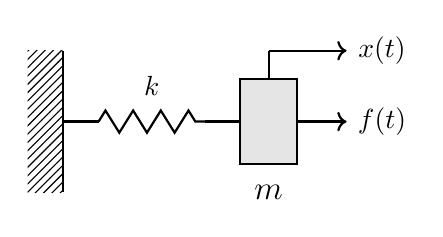
\begin{tikzpicture}[scale=0.9]
                % 固定壁
                \fill[pattern=north east lines] (-0.5,0) rectangle (0,2);
                \draw[thick] (0,0) -- (0,2);
            
                % バネ
                \draw[thick] (0,1) -- (0.5,1);
                \draw[thick, decorate, decoration={zigzag, segment length=10, amplitude=4}] (0.5,1) -- (2,1);
                \node at (1.25,1.5) {$k$};
            
                % --- 物体 ---
                \draw[thick] (2,1) -- (2.5,1); % 棒(変更なし)
                \draw[thick, fill=gray!20] (2.5,0.4) rectangle (3.3,1.6); % 筒の側面
                \node at (2.9,0) {\large $m$};
        
        
                % 入力矢印
                \draw[->, thick] (3.3,1.0) -- (4.0,1.0);
                \node at (4.5,1.0) {$f(t)$};
            
                % 出力矢印
                \draw[thick] (2.9,1.6) -- (2.9,2.0);
                \draw[->, thick] (2.9,2.0) -- (4.0,2.0);
                \node at (4.5,2.0) {$x(t)$};
            

            \end{tikzpicture}
    \end{minipage}
\hfill
    \begin{minipage}[t]{0.3\linewidth}
    (2)\\
        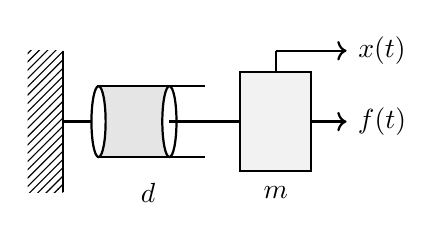
\begin{tikzpicture}[scale=0.9]
            % 固定壁
            \fill[pattern=north east lines] (-0.5,0) rectangle (0,2);
            \draw[thick] (0,0) -- (0,2);
        
            % ダンパー(シリンダー形式)
            \draw[thick] (0,1) -- (0.5,1); % 棒
            \draw[thick, fill=gray!20] (0.5,0.5) rectangle (1.5,1.5); % 筒の側面
            \draw[thick] (1.5,1.5) -- (2,1.5); % 筒の上
            \draw[thick] (1.5,0.5) -- (2,0.5); % 筒の下
            \draw[thick, fill=white] (0.5,1) ellipse (0.1 and 0.5); % 左端面
            \draw[thick, fill=white] (1.5,1) ellipse (0.1 and 0.5); % 右端面
            \draw[thick] (1.5,1) -- (2.5,1); % ピストン棒
            \node at (1.2,0) {$d$};
        
            % 質量M
            \draw[thick, fill=gray!10] (2.5,0.3) rectangle (3.5,1.7);
            \node at (3,0) {$m$};        
            % 座標
            \draw[thick] (3.0,1.7) -- (3.0,2.0);
            \draw[->, thick] (3.0,2.0) -- (4.0,2.0);
            \node at (4.5,2.0) {$x(t)$};
        
            % 外力
            \draw[->, thick] (3.5,1) -- (4.0,1);
            \node at (4.5,1) {$f(t)$};
        \end{tikzpicture}
    \end{minipage}
\hfill
\begin{minipage}[t]{0.3\linewidth}
    (3)\\
    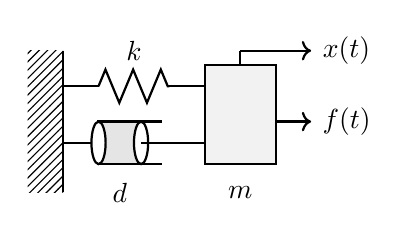
\begin{tikzpicture}[scale=0.9]
            % 固定壁
            \fill[pattern=north east lines] (-0.5,0) rectangle (0,2);
            \draw[thick] (0,0) -- (0,2);
        
            % バネ
            \draw[thick] (0,1.5) -- (0.5,1.5);
            \draw[thick, decorate, decoration={zigzag, segment length=10, amplitude=6}] (0.5,1.5) -- (1.5,1.5);
            \draw[thick] (1.5,1.5) -- (2.0,1.5);
            \node at (1.0,2.0) {$k$};
        
            % ダンパー(シリンダー形式)
            \draw[thick] (0,0.7) -- (0.5,0.7); % 棒
            \draw[thick, fill=gray!20] (0.5,0.4) rectangle (1.1,1.0); % 筒の側面
            \draw[thick] (1.1,1.0) -- (1.4,1.0); % 筒の上
            \draw[thick] (1.1,0.4) -- (1.4,0.4); % 筒の下
            \draw[thick, fill=white] (0.5,0.7) ellipse (0.1 and 0.3); % 左端面
            \draw[thick, fill=white] (1.1,0.7) ellipse (0.1 and 0.3); % 右端面
            \draw[thick] (1.1,0.7) -- (2.0,0.7); % ピストン棒
            \node at (0.8,0) {$d$};
        
            % 質量M
            \draw[thick, fill=gray!10] (2,0.4) rectangle (3,1.8);
            \node at (2.5,0) {$m$};

            % 座標
            \draw[thick] (2.5,1.8) -- (2.5,2.0);
            \draw[->, thick] (2.5,2.0) -- (3.5,2.0);
            \node at (4,2.0) {$x(t)$};
        
            % 外力
            \draw[->, thick] (3,1) -- (3.5,1);
            \node at (4.0,1.0) {$f(t)$};
    \end{tikzpicture}
\end{minipage}

% ---------------[7]---------------
7.下図で表される物理モデルに対する微分方程式を求めよ。\\

\vspace{2mm}

\begin{minipage}[t]{0.45\linewidth}
    (1)\\
        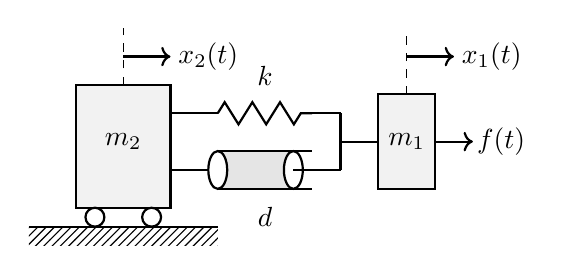
\begin{tikzpicture}[scale=1.2]
            % 質量m2
            \draw[thick, fill=gray!10] (-1,0.4) rectangle (0,1.7);
            \node at (-0.5,1.1) {$m_2$};
            % ローラー追加
            \draw[thick] (-0.8,0.3) circle (0.1);
            \draw[thick] (-0.2,0.3) circle (0.1);

            % 床
            \draw[thick] (-1.5,0.2) -- (0.5,0.2);
            \fill[pattern=north east lines] (-1.5,0) rectangle (0.5,0.2);

            % バネ
            \draw[thick] (0,1.4) -- (0.5,1.4);
            \draw[thick, decorate, decoration={zigzag, segment length=10, amplitude=4}] (0.5,1.4) -- (1.5,1.4);
            \draw[thick] (1.5,1.4) -- (1.8,1.4);
            \node at (1.0,1.8) {$k$};
        
            % ダンパー(シリンダー形式)
            \draw[thick] (0,0.8) -- (0.5,0.8); % 棒
            \draw[thick, fill=gray!20] (0.5,0.6) rectangle (1.3,1.0); % 筒の側面
            \draw[thick] (1.3,1.0) -- (1.5,1.0); % 筒の上
            \draw[thick] (1.3,0.6) -- (1.5,0.6); % 筒の下
            \draw[thick, fill=white] (0.5,0.8) ellipse (0.1 and 0.2); % 左端面
            \draw[thick, fill=white] (1.3,0.8) ellipse (0.1 and 0.2); % 右端面
            \draw[thick] (1.3,0.8) -- (1.8,0.8); % ピストン棒
            \node at (1.0,0.3) {$d$};

            %接続部分
            \draw[thick] (1.8,1.4) -- (1.8,0.8);
            \draw[thick] (1.8,1.1) -- (2.2,1.1);
        
            % 質量m1
            \draw[thick, fill=gray!10] (2.2,0.6) rectangle (2.8,1.6);
            \node at (2.5,1.1) {$m_1$};

        
            % 座標
            \draw[dashed] (-0.5,1.7) -- (-0.5,2.3);
            \draw[->, thick] (-0.5,2.0) -- (0,2.0);
            \node at (0.4,2.0) {$x_2(t)$};

            \draw[dashed] (2.5,1.6) -- (2.5,2.3);
            \draw[->, thick] (2.5,2.0) -- (3.0,2.0);
            \node at (3.4,2.0) {$x_1(t)$};

            \draw[->, thick] (2.8,1.1) -- (3.2,1.1);
            \node at (3.5,1.1) {$f(t)$};




        \end{tikzpicture}
\end{minipage}
\hfill
\begin{minipage}[t]{0.45\linewidth}
    (2)\\
        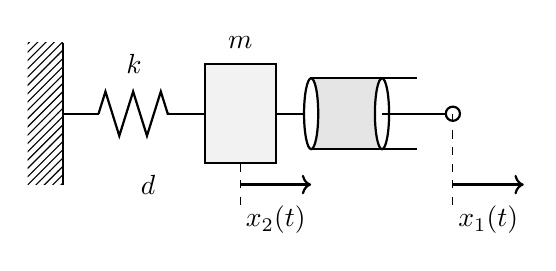
\begin{tikzpicture}[scale=0.9]
            % 固定壁
            \fill[pattern=north east lines] (-0.5,0) rectangle (0,2);
            \draw[thick] (0,0) -- (0,2);
            
            % バネ
            \draw[thick] (0,1.0) -- (0.5,1.0);
            \draw[thick, decorate, decoration={zigzag, segment length=10, amplitude=8}] (0.5,1.0) -- (1.5,1.0);
            \draw[thick] (1.5,1.0) -- (2.0,1.0);
            \node at (1.0,1.7) {$k$};
            
            % 質量M
            \draw[thick, fill=gray!10] (2.0,0.3) rectangle (3.0,1.7);
            \node at (2.5,2.0) {$m$}; 

            % ダンパー(シリンダー形式)
            \draw[thick] (3.0,1) -- (3.5,1); % 棒
            \draw[thick, fill=gray!20] (3.5,0.5) rectangle (4.5,1.5); % 筒の側面
            \draw[thick] (4.5,1.5) -- (5.0,1.5); % 筒の上
            \draw[thick] (4.5,0.5) -- (5.0,0.5); % 筒の下
            \draw[thick, fill=white] (3.5,1) ellipse (0.1 and 0.5); % 左端面
            \draw[thick, fill=white] (4.5,1) ellipse (0.1 and 0.5); % 右端面
            \draw[thick] (4.5,1) -- (5.4,1); % ピストン棒
            \node at (1.2,0) {$d$};



            \draw[thick] (5.5,1) circle (0.1);

            % 座標x_1
            \draw[dashed] (5.5,1) -- (5.5,-0.3);
            \draw[->, thick] (5.5,0) -- (6.5,0);
            \node at (6,-0.5) {$x_1(t)$};
            
            % 座標x_2
            \draw[dashed] (2.5,0.3) -- (2.5,-0.3);
            \draw[->, thick] (2.5,0) -- (3.5,0);
            \node at (3,-0.5) {$x_2(t)$};







        \end{tikzpicture}
\end{minipage}

% ---------------[8]---------------
8.次の伝達関数で表されるシステムの単位ステップ応答を求めよ。\\
\[
(1) \quad G(s) = \frac{s+4}{(s+1)(s+2)} \qquad
(2) \quad G(s) = \frac{2}{(s+1)^2} \qquad
(3) \quad G(s) = \frac{5}{s^2+2s+5}
\]


\end{document}